\documentclass{article}

% ============================================================
% NeurIPS 2026 submission: Stage F (cross-modal valence conflict)
% v2 — integrates minimal-pair control, cross-image patching,
% LLaVA boundary condition; reframes headline statistics and
% mechanism claims per internal review.
% Track: main/workshop, double-blind (default option).
% ============================================================
\usepackage{neurips_2026}

\usepackage[utf8]{inputenc}
\usepackage[T1]{fontenc}
\usepackage{hyperref}
\usepackage{url}
\usepackage{booktabs}
\usepackage{amsfonts}
\usepackage{amsmath}
\usepackage{nicefrac}
\usepackage{microtype}
\usepackage{xcolor}
\usepackage{graphicx}

\newcommand{\todo}[1]{\textcolor{red}{[TODO: #1]}}
\newcommand{\gemma}{Gemma-3-4B}
\newcommand{\gemmabig}{Gemma-3-12B}
\newcommand{\qwen}{Qwen3-VL-8B}
\newcommand{\llava}{LLaVA-1.5-7B}
\newcommand{\betaimg}{\beta_{\text{img}}}
\newcommand{\betatxt}{\beta_{\text{txt}}}

\title{Negative Words Defeat Positive Images: Valence-Asymmetric Conflict Resolution in Vision-Language Models}

\author{%
  Anonymous Author(s) \\
  Anonymous Affiliation \\
  \texttt{anon@example.com} \\
}

\begin{document}

\maketitle

\begin{abstract}
When an image and its accompanying text disagree, a vision-language model (VLM) must decide which to believe. Prior work asks \emph{which modality} wins such conflicts; we ask whether the answer depends on \emph{what the text says}. We pair emotionally positive and negative photographs of people with short context sentences of the opposite valence and measure, against neutral-context baselines, how far each cue moves the model's emotion judgment. In \gemma{}, conflict resolution is strongly asymmetric: a single negative sentence overrides a positive image on $84\%$ of trials, while a positive sentence overrides a negative image on only $21\%$. The asymmetry survives token-matched minimal pairs that differ by one word (\emph{won} vs.\ \emph{lost}), so it tracks valence rather than event content, and it appears only when the image is present. It replicates on \qwen{} and \gemmabig{} but is absent on \llava{}, whose judgments remain anchored to the image. Activation patching traces both the text's and the image's valence signal to a shared set of text-token states in the language stack, where a valence direction learned purely from text causally shifts conflict outcomes. The valence of competing evidence, and the architecture that merges the modalities, are first-class variables in multimodal conflict resolution.
\end{abstract}

\section{Introduction}
\label{sec:intro}

Show a vision-language model a smiling face alongside the sentence \emph{``This was taken at her best friend's funeral,''} and it must decide which signal to believe. A growing literature establishes that VLMs can follow either modality when the two disagree, with the preference swinging by task, model, and prompt \citep{deng2025blindfaith, mixedsignals2025, contextvqa2026, signpost2026}. But this work treats the two competing signals as interchangeable content: it asks \emph{which modality} wins, not whether the outcome depends on \emph{what} the competing evidence says.

We ask a sharper question: does cross-modal conflict resolution depend on the valence of the competing information? Human affective science suggests it should. Negativity dominance --- the finding that mixtures of negative and positive cues are judged more negatively than their parts predict --- is among the most replicated results in psychology \citep{rozin2001, baumeister2001}, and context sentences are known to reshape how people read facial emotion \citep{aviezer2008, aviezer2012}. Whether VLMs show an analogous asymmetry, in which models, and through what computation, has not been established.

Our paradigm is simple. We take photographs of people from the extremes of the EMOTIC valence distribution \citep{kosti2019} and pair each with one-sentence contexts --- positive, negative, and neutral --- inserted into a fixed prompt that asks what the person is feeling. Both conflict directions are run (negative sentence on a positive image, and the mirror), and every effect is measured against the neutral-context baseline. We read the model's judgment two ways: behaviorally, from the probabilities it assigns to emotion words; and internally, with a linear valence probe trained only on text \citep{tak2025} and applied, frozen, under image input.

Four findings emerge.
\begin{enumerate}
  \item \textbf{Conflict resolution is valence-asymmetric (\gemma{}).} A negative sentence overrides a positive image on $84\%$ of trials; a positive sentence overrides a negative image on $21\%$ (gap $+64\%$, 95\% CI $[+55, +72]$). On the graded readout, the negative-context shift is ${\sim}1.8\times$ larger than its mirror ($-0.598$ vs.\ $+0.333$; contrast $+0.265$, CI $[+0.095, +0.431]$).
  \item \textbf{The asymmetry tracks valence, not event content.} Six minimal pairs --- sentences identical up to one valence word (won$\leftrightarrow$lost, wonderful$\leftrightarrow$devastating) --- reproduce the override gap ($+65\%$ vs.\ $+64\%$). Without the image the two context banks are roughly equally strong; the asymmetry appears only when the image is present.
  \item \textbf{The effect is architecture-dependent.} It replicates on \qwen{} (gap $+39\%$) and persists from \gemma{} to \gemmabig{}, but is \emph{absent} on \llava{} (gap $-13\%$): the strongly image-anchored linear-projector design resists textual override in both directions.
  \item \textbf{Both cues converge on a shared channel (\gemma{}).} Activation patching shows the context's valence signal is carried by downstream text-token states, not image tokens; and the image's own valence, initially in the image tokens, migrates into those same text positions over depth. The two cues therefore compete in one text-stream channel --- where negative language wins --- and a valence direction learned purely from text, injected there, causally shifts conflict outcomes (slope $+0.215$).
\end{enumerate}

Our contributions:
\begin{itemize}
  \item \textbf{Phenomenon.} A controlled demonstration that cross-modal conflict resolution is valence-asymmetric, measured in both conflict directions against neutral baselines, with saturation and floor effects explicitly controlled (\S\ref{sec:conflict}).
  \item \textbf{Valence specificity.} A token-matched minimal-pair control that separates valence from event content, including a stricter within-item test that we report as positive but marginal (\S\ref{sec:minimal}).
  \item \textbf{Architecture dependence.} The effect holds on two of the three vision-language designs we test (Gemma-3, Qwen3-VL) and is absent on the third (\llava{}), making image-anchoring a boundary condition rather than assuming the effect is universal (\S\ref{sec:models}).
  \item \textbf{Mechanism.} Patching experiments locate the context's valence signal in downstream text-token states and show the image's valence migrating into those same states, yielding a shared-channel account of the competition (\S\ref{sec:mechanism}).
\end{itemize}

We scope our claims carefully. We do not claim to discover that text can override vision \citep{deng2025blindfaith, contextvqa2026}, nor the first mechanistic study of multimodal conflict \citep{seeingoverrides2026}, nor the first study of multimodal emotion conflict \citep{mosear2025}. And while the behavioral pattern is consistent with negativity dominance in humans, we treat it as an analogue, not the same construct.

\section{Related work}
\label{sec:related}

\paragraph{Modality conflict in VLMs.}
Several lines of work create mismatched image-text pairs and ask which modality the model follows. \citet{deng2025blindfaith} show VLMs disproportionately trust text under corrupted-text conflicts; \citet{mixedsignals2025} find the preferred modality swings with task complexity and model; \citet{contextvqa2026} report that contradictory persuasive text overrides clear visual evidence across 11 VLMs; \citet{signpost2026} extend this to geolocation; and \citet{camel2025} find misleading instructions become \emph{more} influential when an image is present. These studies establish text-vision conflict as real and safety-relevant, but treat the competing content as interchangeable. We add two axes: valence (controlled conflicts in both directions, with text-only strength checks) and architecture (the same conflict battery yields opposite outcomes on \llava{} versus Gemma/Qwen).

\paragraph{A conflict-type taxonomy.}
A complementary mechanistic literature studies conflicts between visual input and the model's \emph{internal parametric knowledge}: \citet{nooralahzadeh2026} find image tokens carry nearly all causal impact when a model must override its prior; \citet{lietzow2026} identify sparse late attention heads governing prior override; \citet{seeingoverrides2026} causally steer such conflicts. These results do not contradict ours. In image-vs.-prior conflicts the competing signal lives in the weights; in our image-vs.-external-text conflicts it arrives in the prompt and is carried by the text stream. Our cross-image result adds a wrinkle: in \gemma{}, even the \emph{image's} decision-relevant signal migrates into text positions over depth, so where a conflict is resolved depends jointly on conflict type, depth, and architecture.

\paragraph{Emotion and affect in multimodal models.}
EMOTIC and related corpora have been used to benchmark VLM emotion recognition \citep{kosti2019, etesam2024, agarwal2026}, and emotion conflicts across audio-visual modalities have been benchmarked \citep{mosear2025, emomm2026}. VEENA \citep{veena2026} identifies emotion circuits in LVLMs and intervenes to improve recognition; it studies congruent emotion processing with no modality conflict and no valence asymmetry. In text-only LLMs, \citet{tak2025} localize appraisal representations and steer emotion inference causally (our methodological foundation), and \citet{negbeforepos2026} report asymmetric valence processing across layers, an LLM-internal precedent that our cross-modal, behavioral-override setting extends.

\paragraph{Mechanistic interpretability of VLMs.}
Activation patching and causal tracing are established tools \citep{meng2022, patchingbestpractices, attributionpatching}, and cross-modal information flow has been traced in VLMs: image information transfers into text/query positions in early-to-middle layers \citep{basu2024, whatsintheimage2025, narrowgate2024, towardsinterp2024}, and middle-layer last-token attention matters for cross-modal aggregation \citep{fcct2026}. Our cross-image migration result (\S\ref{sec:crosspatch}) is consistent with this literature; our contribution is the conflict-specific decomposition, not the existence of image-to-text transfer. \citet{nikankin2025} find largely disjoint circuits for analogous visual and textual tasks; this is compatible with our claims, since we posit a shared valence-sensitive channel within the language backbone, not a single modality-agnostic circuit. Work on attention sinks and delimiter tokens \citep{xiao2024, activedormant2024}, and on safety signals concentrating in assistant header tokens \citep{zhang2026anydepth}, anticipates structural tokens as aggregation sites. Our carrier in \gemma{} is the assistant-turn boundary, not the BOS sink, though a generic-bottleneck interpretation is not yet excluded (\S\ref{sec:patching}).

\paragraph{Human affective science.}
Negativity dominance \citep{rozin2001} and ``bad is stronger than good'' \citep{baumeister2001} are foundational asymmetries in human evaluation, and situational sentences modulate facial-affect perception \citep{aviezer2008, aviezer2012}. We use this literature as motivation; whether VLM valence asymmetries share anything computational with the human construct is an open question our operationalization (cross-modal override) does not settle.

\paragraph{Steering vectors.}
Difference-of-means steering is causally effective but its interpretation requires care \citep{steeringunreliability2025, steeringnonident2026}. We pre-empt standard concerns with norm-matched random nulls and a non-valence specificity control, and we deliberately describe our steering result as causal \emph{outcome control} under conflict, not as re-weighting of the competing cues (\S\ref{sec:arbitration}).

\section{Experimental framework}
\label{sec:setup}

\paragraph{Task and stimuli.}
Each trial shows the model one photograph of a person together with a one-sentence context, inside a fixed prompt that asks \emph{``What single emotion is this person feeling?''} (exact template in Appendix~\ref{app:contexts}). The images are the 75 most positive and 75 most negative person annotations from the EMOTIC test split \citep{kosti2019} (150 persons across 121 distinct images). The contexts come in two banks: a \emph{full bank} of 6 positive, 6 negative, and 2 neutral generic sentences (``This photo was taken moments after they won the championship.''), and a \emph{minimal-pair bank} of 6 sentence pairs that are identical except for one valence-bearing word (won$\leftrightarrow$lost; token counts matched per pair on the Gemma tokenizer, so the readout position is identical within each pair; Appendix~\ref{app:contexts}). Crossing images with contexts gives 15 conditions per image, 2{,}250 forward passes per bank. EMOTIC annotates emotions per person but we feed whole images without bounding boxes, so target ambiguity is a real concern; we quantify it: exactly one of the 121 images contains annotated persons in both extreme groups, and excluding it barely moves the headline contrast ($+0.330 \to +0.312$ on the minimal-pair bank). Marked-person reruns remain future work (\S\ref{sec:limitations}).

\paragraph{Design decisions.}
Two choices matter for interpreting everything that follows. First, all effects are measured against the \emph{neutral-context} baseline, not the bare no-context prompt: adding any framing sentence, even a neutral one, shifts the model's judgment by itself (Appendix~\ref{app:nocontext}), so we hold the presence of a sentence constant and vary only its polarity. Second, we use \emph{banks} of contexts rather than single sentences: an early single-sentence pilot produced conclusions that did not survive the bank design (Appendix~\ref{app:pilot}).

\paragraph{Models.}
Primary model: \texttt{google/gemma-3-4b-it} (34 layers, $d_{\text{model}}{=}2560$; SigLIP vision tower pooled to 256 image tokens), accessed via TransformerBridge in bf16. To test generality we use three further models spanning distinct vision-language designs: \qwen{} (native dynamic-resolution ViT), \llava{} (frozen CLIP ViT through a linear projector, unpooled patch tokens), and \gemmabig{} (scale within family). All measurements are single forward passes; nothing is generated. Compute details are in Appendix~\ref{app:compute}.

\paragraph{Behavioral readouts.}
We read the model's judgment from the probabilities it assigns to 13 emotion words (\emph{joy}, \emph{sadness}, \emph{fear}, \ldots; full list and polarity grouping in Appendix~\ref{app:contexts}) at the last prompt token. \emph{Behavioral valence} is $P(\text{positive labels}) - P(\text{negative labels})$, a graded score in $[-1, 1]$. For comparisons across models we use the \emph{override rate}: the fraction of conflict trials where the model's top emotion label follows the text rather than the image. The override rate needs no calibration across models, which matters because behavioral valence is bounded and each model occupies the scale differently. Where the graded score approaches its floor or ceiling we report saturation-corrected (head-room-normalized) effects, and we interpret only relative shifts; an unbounded logit-margin variant is future work (\S\ref{sec:limitations}).

\paragraph{Internal readout.}
Alongside behavior, we read the model's internal state with a linear \emph{pleasantness} probe: a ridge regression trained on text-only activations (crowd-enVENT \citep{troiano2023}, \texttt{attn\_out} layer 18, last token), following \citet{tak2025}. The probe is frozen after text training and never re-fit on image data, so anything it reads under image input reflects a representation shared across modalities. It tracks EMOTIC ground-truth valence at $\rho = 0.507$ under image conditioning (\S\ref{sec:foundations}). We call what it reads a valence-sensitive channel, not \emph{the} valence representation: the probe direction reads but does not steer, while a difference-of-means direction in the same space steers.

\section{A shared cross-modal valence readout and a causal handle}
\label{sec:foundations}

Before studying conflicts, we establish that image and text share a valence representation the model actually uses; full details are in Appendix~\ref{app:foundations}. Three facts carry over. \textbf{(1) A text-trained probe localizes valence.} Following \citet{tak2025}, ridge probes for six appraisal dimensions peak mid-network (layers 17--21 of 34) at the attention output, far above shuffled baselines; pleasantness is strongest (validation $r^2 = 0.641$ at layer 18), and layer 18 is fixed as the readout and steering site for everything that follows. \textbf{(2) The probe transfers to images.} Applied unchanged to image-conditioned activations, it tracks EMOTIC valence at Spearman $\rho = +0.507$ ($n{=}7{,}280$; polarity AUC $0.898$), beats all of 100 norm-matched random directions ($p{=}0.010$), and keeps a unique contribution after controlling for what the model would say in captions (semipartial $\rho = +0.201$, $p{<}0.001$) --- so the shared representation is not just internal verbalization. \textbf{(3) The channel is causal.} A difference-of-means pleasantness direction estimated purely from text, injected at layer 18 under image input, moves behavioral valence monotonically (slope $+0.329$), ${\sim}12\times$ a random null and ${\sim}4.5\times$ a non-valence control direction. Image and text thus both write into a shared, causally manipulable valence channel in the language backbone; the computation upstream of it may still be modality-specific \citep{nikankin2025}.

\section{Valence-asymmetric conflict resolution}
\label{sec:conflict}

\subsection{Balanced integration under conflict}
\label{sec:integration}

Before asking who wins a conflict, we check that both cues matter at all. Regressing each readout on image valence and context polarity (both z-scored; sentence-bearing conditions only) shows both cues enter with the correct sign and comparable weight (Table~\ref{tab:integration}); text slightly leads the behavioral output ($|\betatxt|/|\betaimg| = 1.19$, and the minimal-pair bank replicates this at $1.19$). Neither modality is ignored, so the asymmetry below is a fact about how conflicts are \emph{resolved}, not about one cue being unheard. We scope this balance to the affective-context regime we test.

\begin{table}[t]
  \caption{Modality integration under conflict (\gemma{}, full bank). Both cues are sign-correct and comparable, which makes the asymmetry below an arbitration result rather than a triviality.}
  \label{tab:integration}
  \centering
  \begin{tabular}{lrrr}
    \toprule
    Readout & $\betaimg$ & $\betatxt$ & $|\betatxt|/|\betaimg|$ \\
    \midrule
    Frozen pleasantness probe (attn\_out L18) & $+0.367$ & $+0.315$ & $0.86$ \\
    Behavioral valence (logits)               & $+0.322$ & $+0.382$ & $1.19$ \\
    \bottomrule
  \end{tabular}
\end{table}

\subsection{The asymmetry: the full factorial picture}
\label{sec:asymmetry}

Table~\ref{tab:factorial} reports the complete image-polarity $\times$ context-polarity matrix. The \textbf{primary contrast is between the two conflict cells}, which mirror each other by design. A negative sentence moves positive-image judgments by $-0.598$; the mirror move, a positive sentence on negative images, is $+0.333$. We call the difference in their magnitudes the \emph{mirror contrast}: $+0.265$ (bootstrap 95\% CI $[+0.095, +0.431]$; Mann-Whitney $p = 0.005$), a ${\sim}1.8\times$ ratio. Because negative images sit closer to the scale floor, we also normalize each move by the room it had to travel; the asymmetry survives (normalized pulls $0.632$ vs.\ $0.259$), so it is not a floor artifact. In categorical terms: negative context overrides a positive image on $84\%$ of trials, positive context overrides a negative image on $21\%$ (gap $+64\%$, 95\% CI clustered over images $[+55, +72]$).

A second, distinct comparison stays \emph{within} the positive-image row, where the neutral baseline sits mid-scale ($-0.058$) and the room to move is symmetric: negative and positive contexts differ $3.58\times$ in displacement from neutral ($-0.598$ vs.\ $+0.167$). Note what this ratio is and is not: it compares a conflicting against an \emph{agreeing} context on the same image, so it measures how unequal the two polarities' leverage is, not the mirror override, and we report it separately. It can also mislead on its own: \llava{} shows $3.06\times$ purely from ceiling/floor geometry while its mirror contrast is null (\S\ref{sec:models}).

\begin{table}[t]
  \caption{Full factorial matrix (\gemma{}, full bank): mean behavioral valence per cell, and the effect vs.\ the neutral baseline in parentheses. The mirror contrast compares the two incongruent cells (bold); the within-positive-image $3.58\times$ compares the bold and italic cells of the first row.}
  \label{tab:factorial}
  \centering
  \begin{tabular}{lccc}
    \toprule
    & Positive context & Neutral context & Negative context \\
    \midrule
    Positive image & \emph{$+0.109$ ($+0.167$)} & $-0.058$ (baseline) & $\mathbf{-0.656}$ ($\mathbf{-0.598}$) \\
    Negative image & $\mathbf{-0.473}$ ($\mathbf{+0.333}$) & $-0.806$ (baseline) & $-0.862$ ($-0.056$) \\
    \bottomrule
  \end{tabular}
\end{table}

\subsection{Valence, not event semantics: token-matched minimal pairs}
\label{sec:minimal}

Could the asymmetry come from the sentences rather than their valence? Text-only, the two full banks are similar in mean strength ($+0.706$ vs.\ $-0.752$; we do not claim statistical equivalence from a non-significant test at $n{=}6$ sentences per polarity). But similar strength does not rule out the strongest alternative: ``funeral'' and ``championship'' describe different \emph{events}, and some events point to emotion labels more directly than others. We therefore built six \emph{minimal pairs}: sentences identical except for one valence-bearing word (won$\leftrightarrow$lost, best$\leftrightarrow$worst, got$\leftrightarrow$lost, wonderful$\leftrightarrow$devastating, celebration$\leftrightarrow$memorial, joyful$\leftrightarrow$heartbreaking), with token counts verified equal within each pair on the Gemma tokenizer so the readout position is identical.

\begin{table}[t]
  \caption{The asymmetry is valence-specific: the token-matched minimal-pair bank reproduces (and if anything sharpens) every headline metric of the full bank.}
  \label{tab:minimal}
  \centering
  \small
  \begin{tabular}{lrr}
    \toprule
    Metric & Full bank & Minimal pairs \\
    \midrule
    Override gap (neg$>$pos img $-$ pos$>$neg img) & $+64\%$ $[+55,+72]$ & $+65\%$ $[+56,+73]$ \\
    Mirror contrast $|$drop$|-|$rise$|$ & $+0.265$ $[+0.095,+0.431]$ & $+0.330$ $[+0.151,+0.501]$ \\
    Head-room-normalized pull (drop / rise) & $0.63$ / $0.26$ & $0.92$ / $0.23$ \\
    Text-only $|$neg$|/|$pos$|$ (no image) & $1.06$ & $1.25$ \\
    Within-positive-image displacement ratio & $3.58$ & $3.56$ \\
    \bottomrule
  \end{tabular}
\end{table}

The effect is unchanged (Table~\ref{tab:minimal}): the override gap is statistically indistinguishable ($+65\%$ vs.\ $+64\%$) and the mirror contrast sharpens under the cleaner control. When the only difference between conditions is a single valence word, the asymmetry holds --- it is about valence, not event content. Text-only, the minimal banks are again similar in strength (ratio $1.25$, slightly above the full bank's $1.06$; this residual imbalance is why we treat the override rate and the head-room-controlled metrics, not raw text-only symmetry, as primary).

\paragraph{The strictest test, reported honestly.}
Minimal pairs allow an even stricter comparison: within each image and each pair, compare the negative member's effect to the positive member's ($|\Delta_{\rm neg}| - |\Delta_{\rm pos}|$, vs.\ that image's neutral baseline, on positive images). This is positive but marginal: $+0.166$, bootstrap CI $[+0.016, +0.324]$, Wilcoxon $p = 0.052$. The per-pair breakdown (Table~\ref{tab:pairs}) shows why, and the reason is itself informative: every negative sentence moves the readout reliably ($-0.35$ to $-0.74$), while positive sentences are hit-or-miss --- two concrete positives break through even against the image, and one pair reverses. Within matched events, the asymmetry comes from the \emph{consistency} of negative framing, not from uniformly larger negative magnitudes. The override gap and mirror contrast remain the primary results; this paired test refines the phenomenon's shape.

\begin{table}[t]
  \caption{Per-pair within-item contrasts (positive images, minimal-pair bank). Negative framing moves the judgment reliably in every pair; positive framing is event-dependent.}
  \label{tab:pairs}
  \centering
  \small
  \begin{tabular}{llrrr}
    \toprule
    Pair & Swap & $\Delta_{\rm neg}$ & $\Delta_{\rm pos}$ & $|\Delta_{\rm neg}|-|\Delta_{\rm pos}|$ \\
    \midrule
    mp0 & won $\leftrightarrow$ lost & $-0.547$ & $+0.469$ & $+0.078$ \\
    mp1 & best $\leftrightarrow$ worst & $-0.534$ & $-0.055$ & $+0.479$ \\
    mp2 & got $\leftrightarrow$ lost & $-0.658$ & $-0.264$ & $+0.394$ \\
    mp3 & wonderful $\leftrightarrow$ devastating & $-0.742$ & $+0.285$ & $+0.457$ \\
    mp4 & celebration $\leftrightarrow$ memorial & $-0.348$ & $+0.453$ & $-0.105$ \\
    mp5 & joyful $\leftrightarrow$ heartbreaking & $-0.413$ & $+0.215$ & $+0.198$ \\
    \bottomrule
  \end{tabular}
\end{table}

\paragraph{The image creates the asymmetry.}
With no image, the banks are near-symmetric. Add a positive image, and only $24\%$ of the positive-text effect survives while $80\%$ of the negative-text effect does: the image selectively suppresses the framing that \emph{agrees} with it. The asymmetry is therefore a cross-modal phenomenon, not a property of the sentences. We present this as a strong descriptive interaction; a formal test propagating uncertainty over images and sentences simultaneously is future work (\S\ref{sec:limitations}).

\begin{figure}[t]
  \centering
  \begin{minipage}[t]{0.49\linewidth}
    \centering
    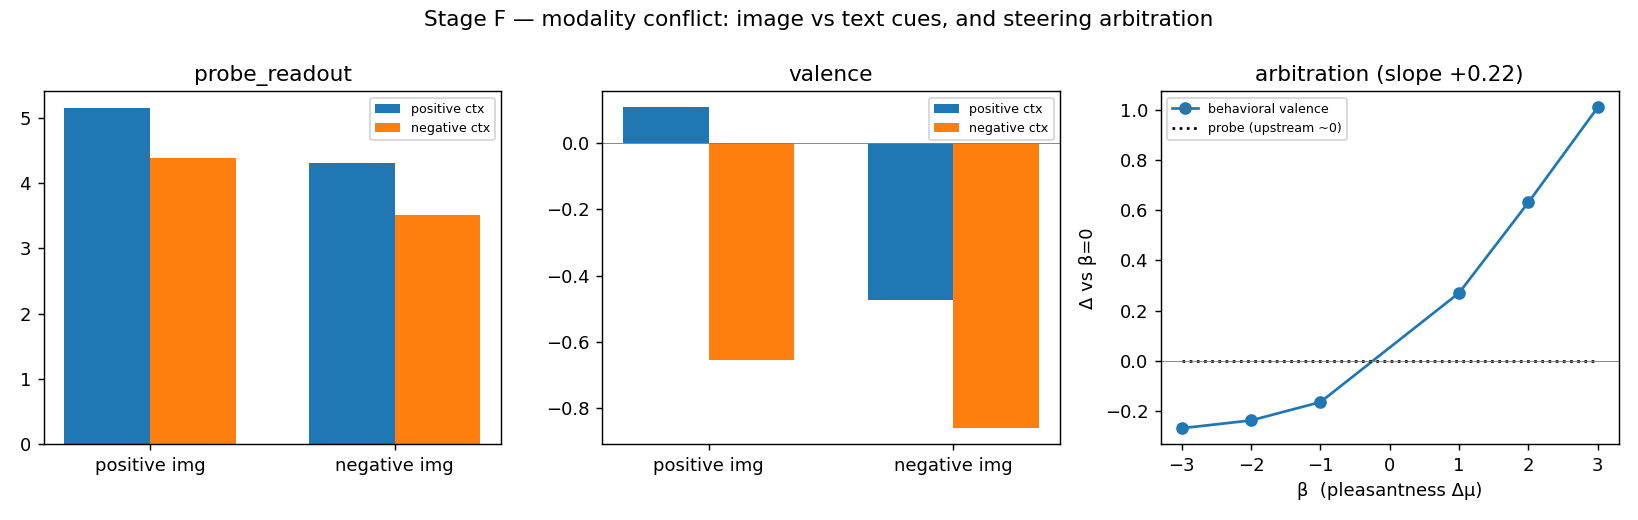
\includegraphics[width=\linewidth]{figures/stage_f_conflict.png}
  \end{minipage}\hfill
  \begin{minipage}[t]{0.49\linewidth}
    \centering
    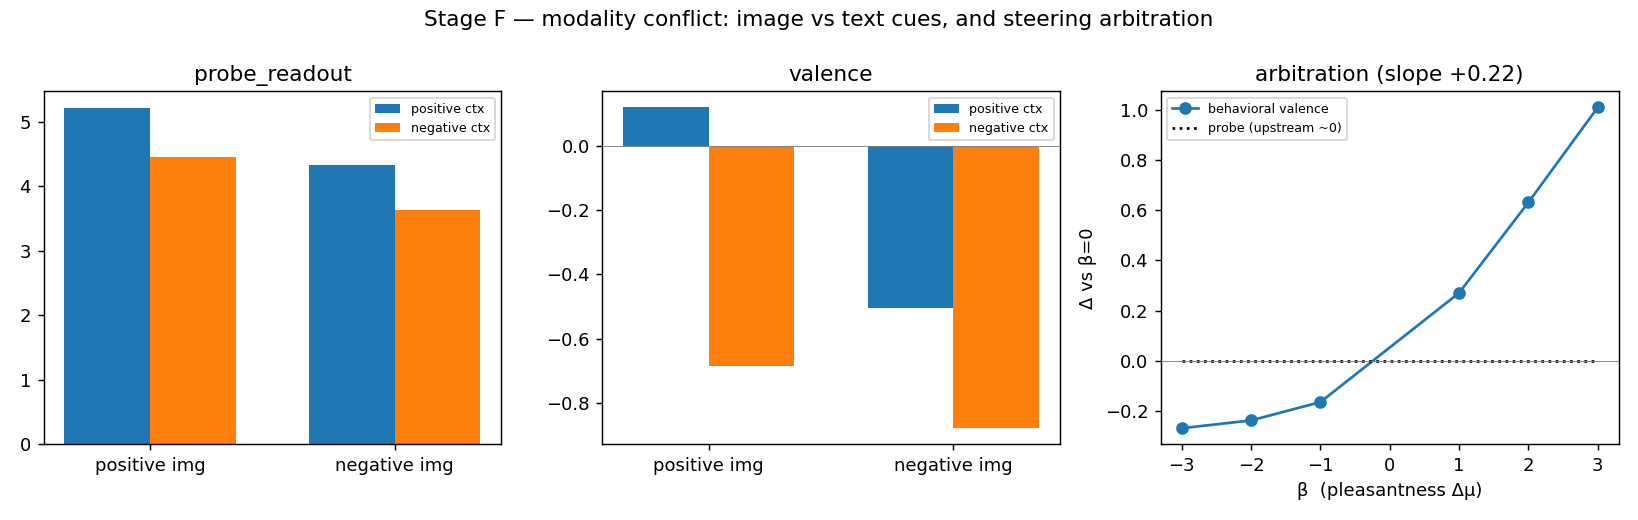
\includegraphics[width=\linewidth]{figures/conflict_minimal.png}
  \end{minipage}
  \caption{Valence-asymmetric conflict resolution on the full bank (\emph{left}) and its replication on the token-matched minimal-pair bank (\emph{right}): behavioral valence per image group and context polarity vs.\ the neutral baseline.}
  \label{fig:conflict}
\end{figure}

\section{Mechanism: a shared text-stream channel}
\label{sec:mechanism}

\subsection{The divergence emerges mid-stack}
\label{sec:layerwise}

Where in the network do positive- and negative-context runs come apart? Projecting every layer's last-token state onto the frozen probe direction (a logit-lens-style diagnostic), the divergence first clears the noise floor around layer 13 of 34 ($|d| = 0.21$; the floor, $0.125$, is estimated from the pre-divergence layers) and then amplifies ${\sim}7\times$ through the back half of the network, peaking near layer 28 ($|d| = 1.47$). We read this as ``detectable mid-stack under this lens,'' not as evidence of where the signal is created. The signal also reaches the readout indirectly: at layer 18 the last token attends ${\sim}88\%$ to template and question tokens and only ${\sim}3.5\%$ to the context itself, whose direct contribution under attention knockout is ${\sim}6\%$ --- so the context's influence must be carried by intermediate positions. The next experiment finds which.

\subsection{Same-image patching: where the context-polarity signal is carried}
\label{sec:patching}

Which token positions carry the context's valence signal? Holding the \emph{image} constant, we take a positive-context run (donor) and a negative-context run (recipient), overwrite the recipient's residual stream over layers 13--17 for one group of token positions at a time, and measure how far the readout recovers toward the donor's. The token whose state is scored is \emph{excluded} from every patched group, so recovery at the assistant-turn boundary is not tautological. Results replicate across two context pairs (Table~\ref{tab:patching}); full methodology in Appendix~\ref{app:patching}.

\begin{table}[t]
  \caption{Same-image patching recovery of the context-induced delta (probe readout, layers 13--17, \gemma{}). The context-polarity signal is carried through downstream text-stream states, concentrated at the assistant-turn boundary; BOS and the user-turn prefix carry none of it.}
  \label{tab:patching}
  \centering
  \small
  \begin{tabular}{lrr}
    \toprule
    Patched group & Pair 1 & Pair 2 \\
    \midrule
    Image tokens                 & $-1\%$ & $+1\%$ \\
    BOS                          & $0\%$  & $-1\%$ \\
    User-turn prefix delimiters  & $0\%$  & $-1\%$ \\
    Question tokens              & $22\%$ & $32\%$ \\
    Assistant-turn boundary      & $\mathbf{65\%}$ & $\mathbf{57\%}$ \\
    All aligned text             & $85\%$ & $87\%$ \\
    \bottomrule
  \end{tabular}
\end{table}

The context's valence signal is thus carried by downstream text-token states, concentrated at the assistant-turn boundary; image tokens and the BOS sink carry none of it. Four caveats bound this conclusion. \textbf{(1)} The experiment localizes where the positive-vs.-negative \emph{difference} travels; it does not by itself explain why the negative direction dominates behaviorally --- a symmetric model could show the same decomposition. \textbf{(2)} The ${\sim}0\%$ image-token recovery is partly guaranteed by causal ordering: the image precedes the context in the prompt, so image-position states cannot depend on it. We treat this row as a consistency check; the direct test is a context-before-image ordering variant, which is future work. \textbf{(3)} The assistant-turn boundary is where a causal LM would be expected to accumulate preceding prompt information anyway, so a generic answer-preparation-bottleneck reading is not excluded; the missing control is a matched non-affective contrast run through the same decomposition. \textbf{(4)} The ${\sim}13$--$15\%$ not recovered by all aligned text is an unrecovered residual under this intervention, not an estimate of the context tokens' causal share; recovery is nonlinear and non-additive (Qwen is super-additive). Finally, the full-bank donor/recipient sentences differ in token length, so aligned positions sit at different absolute offsets; the token-matched minimal pairs remove this confound, and re-running the patching on them is planned.

\subsection{Cross-image patching: visual valence migrates into the text stream}
\label{sec:crosspatch}

The mirror question is where the \emph{image's own} valence lives. Now we hold the context fixed (neutral) and vary the image (donor $=$ positive image, recipient $=$ negative image). The two runs then have byte-identical \texttt{input\_ids}, so every position, including the context, can be patched 1:1. Table~\ref{tab:crosspatch} shows recovery of the image-driven readout gap across three depth bands (behavioral valence; the L18 probe corroborates in the bands where it is valid):

\begin{table}[h]
  \caption{Cross-image patching (\gemma{}, 60 image pairs, neutral context): recovery of the image-driven valence gap by band. Visual valence is recoverable only from image tokens early, and only from text-stream positions late.}
  \label{tab:crosspatch}
  \centering
  \begin{tabular}{lrrr}
    \toprule
    Patch band (layers) & Image tokens & All non-image text & All positions (sanity) \\
    \midrule
    0--12 (early) & $\mathbf{80\%}$ & $10\%$ & $100\%$ \\
    13--17 (mid)  & $66\%$ & $65\%$ & $91\%$ \\
    18--28 (late) & $\mathbf{9\%}$ & $\mathbf{68\%}$ & $79\%$ \\
    \bottomrule
  \end{tabular}
\end{table}

Visual valence \emph{originates} in the image tokens and \emph{broadcasts into the text-stream positions over depth}: by the late band the image tokens no longer carry the decision-relevant signal, and the text-stream states do. This corrects a natural but wrong reading of \S\ref{sec:patching} --- that the image's valence stays confined to image tokens --- and matches the image-to-text transfer literature \citep{basu2024, whatsintheimage2025}. The picture that results is a \emph{shared-channel competition}: both cues are read out from the same downstream text-stream states, and in \gemma{}/\qwen{} negative language wins there. The image loses not because its signal is trapped, but because it is out-competed at the point of aggregation. One question stays open: whether the image still broadcasts \emph{while losing}. A confirmatory run with a fixed \emph{negative} context restates the dominance behaviorally --- the image-driven valence gap collapses from $0.87$ to $0.08$ --- but that same collapse makes late-band recovery denominators near-zero, so broadcast-under-competition could not be localized (mid-band probe recovery from image tokens remains high, $85\%$, CI $[51, 150]$).

\section{Generality, robustness, and causal outcome control}
\label{sec:robustness}

\subsection{Three unification architectures: replication and a boundary}
\label{sec:models}

Is the asymmetry a property of VLMs in general, or of particular designs? We run the identical conflict battery on three ways of connecting vision to language: Gemma-3 (SigLIP tower pooled to 256 soft tokens), \qwen{} (native dynamic-resolution ViT), and \llava{} (frozen CLIP ViT through a linear projector, unpooled patch tokens), scored with the calibration-free override rate (Table~\ref{tab:models}).

\begin{table}[t]
  \caption{The asymmetry is architecture-dependent: it replicates on \qwen{} and is absent on \llava{}. LLaVA's within-positive-image ratio ($3.06\times$) illustrates why that ratio alone is a trap: it arises from ceiling/floor geometry while the head-room-normalized pulls are exactly symmetric and the override gap is slightly \emph{reversed}.}
  \label{tab:models}
  \centering
  \scriptsize
  \setlength{\tabcolsep}{3.5pt}
  \begin{tabular}{lrrr}
    \toprule
    Metric & \gemma{} & \qwen{} & \llava{} \\
    \midrule
    Text-only $|$neg$|/|$pos$|$ (banks matched) & $1.06$ & $1.00$ & $0.99$ \\
    Within-positive-image displacement ratio & $3.58\times$ & $3.64\times$ & $3.06\times$ \\
    Head-room-normalized pull (drop / rise) & $0.63$ / $0.26$ & (saturates) & $0.33$ / $0.33$ \\
    Mirror contrast $|$drop$|-|$rise$|$ & $+0.265$ $[+.10,+.43]$ & $+0.394$ $[+.25,+.54]$ & $-0.018$ $[-.08,+.05]$ \\
    Override gap (95\% CI, clustered) & $+64\%$ $[+55,+72]$ & $+39\%$ $[+30,+49]$ & $\mathbf{-13\%}$ $[-22,-3]$ \\
    \bottomrule
  \end{tabular}
\end{table}

\qwen{} replicates the asymmetry near-quantitatively (its graded valence saturates, so the override rate is the primary cross-model metric; its mirror contrast is $+0.394$). \llava{} shows no trace of the effect. Its judgments stay anchored to the image (neutral-context valence near $\pm 0.72$), conflict resolves symmetrically (normalized pulls $0.33/0.33$; mirror-contrast CI straddles zero), and the override gap is slightly \emph{reversed} ($-13\%$). A candidate explanation is representational: LLaVA's unpooled, frozen-CLIP visual input weights the image heavily enough that text cannot commandeer the readout in either direction. Whatever the cause, the correct scope is clear: the asymmetry holds on the two modern pooled/native-ViT designs and not on the older linear-projector design --- it is a property of (model, conflict) pairs, not of VLMs as a class. The coarse mechanism also replicates on \qwen{}: image tokens are causally inert for the context delta ($0\%$ patching recovery), though the carrier is distributed across text positions (all-text $65\%$) rather than concentrated at Gemma's turn boundary. Mechanism experiments were not run on \llava{}, where there is no dominance to localize.

\subsection{Prompt robustness}
\label{sec:prompts}

Rephrasing the question six natural ways with everything else fixed (13{,}500 forwards), the override gap never flips and every CI clears zero: $+46\%$ to $+74\%$, mean $+58\%$, with the base prompt mid-pack (Appendix~\ref{app:prompts}). The sweep reuses the same context bank, so it establishes robustness to phrasing, not to context sampling.

\subsection{Scale}
\label{sec:scale}

From \gemma{} to \gemmabig{}, the gap remains large ($+51\%$, CI $[+0.42, +0.59]$). Negative override rises ($84\% \to 93\%$) and positive override more than doubles ($19\% \to 42\%$): the larger model is more text-driven in \emph{both} directions. Because the two gap CIs overlap and the negative rate is near ceiling at $93\%$, we do not claim the asymmetry itself changes with scale (Appendix~\ref{app:scale}).

\subsection{Steering causally shifts conflict outcomes}
\label{sec:arbitration}

Finally, the shared channel is a causal handle on conflicts, not just a readout. Injecting the text-derived pleasantness direction at layer 18 during conflict trials drives behavioral valence through the conflict at slope $+0.215$ per unit of steering strength --- about $65\%$ of the no-conflict slope ($+0.329$). A direction learned purely from text changes the model's judgment in an ongoing cross-modal conflict; no verbalization account explains that. We claim causal \emph{outcome control} and deliberately not more: a generic output-valence direction could shift the final score the same way, so whether steering re-weights the competing cues themselves (changes the override rates or the cue coefficients) is the natural follow-up.

\section{Discussion}
\label{sec:discussion}

\paragraph{A shared-channel account.}
The mechanistic picture that emerged is more interesting than the one we set out to test. Both cues converge on the same downstream text-stream states: the context's polarity signal is carried there (same-image patching), and the image's valence migrates there over depth (cross-image patching). Conflict is resolved \emph{within} this shared channel, and in Gemma/Qwen negative language wins. What our experiments do not yet establish is the computation that privileges the negative direction inside the channel: patching localizes where polarity information travels, not why one polarity dominates. The per-pair analysis hints at the shape --- negative framing is reliable, positive framing is event-dependent. Normalized neutral$\leftrightarrow$polarity patching in both directions would separate asymmetric mediation from asymmetric input, and is the experiment we would run next.

\paragraph{Why would LLaVA differ?}
The boundary condition constrains explanations. Any account that locates the asymmetry purely in language-side training statistics (``negative words are more diagnostic'') must explain why LLaVA, whose language backbone is trained on the same statistics, shows none of it. The natural hypothesis is that the vision-language design sets the image's weight in the shared channel: LLaVA's unpooled projection keeps the image dominant enough that text cannot override in either direction, while pooled/native-ViT designs admit textual override --- and where override is possible, it is valence-asymmetric. Testing intermediate designs (e.g., LLaVA-NeXT, OneVision) would map the boundary.

\paragraph{Relation to parametric-conflict mechanisms.}
Image-vs.-parametric-knowledge conflicts localize causal load to image tokens \citep{nooralahzadeh2026, lietzow2026}; our external-text conflicts localize the context delta to text states, and even visual valence migrates text-ward by the readout. Conflict type, depth, and architecture jointly determine locus; treating any single localization as universal is unlikely to survive.

\paragraph{Implications.}
Practically: on affect-sensitive tasks, a single negative sentence overrides the visual assessment of a Gemma- or Qwen-class VLM at rates near $90\%$; the text side strengthens with scale; and model choice matters, since an image-anchored design like LLaVA behaves qualitatively differently under identical conflicts. The localization results also suggest concrete monitoring hooks --- the turn-boundary states in Gemma-class models --- where steering demonstrably changes outcomes.

\section{Limitations}
\label{sec:limitations}

\textbf{Mechanism scope.} Our patching localizes where context-polarity information travels, not the computation that makes the negative direction win; the normalized neutral$\leftrightarrow$polarity patching (both directions) has not been run. The ${\sim}0\%$ image-token result for the context delta is partly dictated by causal ordering (image precedes context), and the context-before-image variant has not been run. The assistant-turn-boundary concentration lacks a matched non-affective control, so a generic-bottleneck reading remains open. Full-bank patching pairs are not length-matched; the token-matched minimal pairs enable a clean rerun, which is planned. Broadcast-under-competition could not be localized, because dominance itself collapses the measurable gap.
\textbf{Statistics.} Uncertainty is propagated over images (121 distinct; the one cross-polarity duplicate changes the headline contrast by $0.018$) but not simultaneously over context sentences; a crossed two-way bootstrap is future work, partially mitigated by the minimal-pair within-item test. That within-item contrast is marginal ($p = 0.052$), and two positive pair-members read weak text-only and should be revised. All runs use a single seed.
\textbf{Measurement.} Behavioral valence is a bounded probability score; head-room normalization and the override rate address saturation, but an unbounded logit-margin replication has not been run. EMOTIC persons are fed as whole images without target marking; the duplicate-image check is reassuring, but marked-person or cropped reruns are the direct fix.
\textbf{Scope.} One dataset and task family (person-emotion labeling), one context style, three architectures, with the mechanism probed on one (coarsely on a second). Claims are scoped to controlled image-context emotion judgments on the tested designs; broader conflict domains, tasks, and architectures are open.

\section{Conclusion}
\label{sec:conclusion}

Cross-modal conflict resolution in the VLMs we test is valence-asymmetric: negative language changes image-grounded emotion judgments far more than positive language does. The asymmetry survives token-matched minimal pairs, appears only in the presence of the image, and depends on the architecture --- present in Gemma-3 and Qwen3-VL, absent in image-anchored LLaVA-1.5. Mechanistically, both cues converge on a shared text-stream readout channel in \gemma{}: the context's polarity signal is carried there, the image's valence migrates there over depth, and a valence direction learned purely from text, injected into that channel, causally shifts conflict outcomes. The valence of competing evidence, and the architecture that merges the modalities, are first-class variables in multimodal conflict resolution.

% ============================================================
\begin{ack}
Hidden in the anonymized submission via the ack environment. \todo{Camera-ready: acknowledge mentor/collaborators and the Algoverse program; declare funding and competing interests per \url{https://neurips.cc/Conferences/2026/PaperInformation/FundingDisclosure}.}
\end{ack}

% ============================================================
\bibliographystyle{plainnat}
\bibliography{references}

% ============================================================
\appendix

\section{Foundations: Stages A, C, D in full}
\label{app:foundations}

\subsection{Text-side appraisal probes and steering}
Ridge probes on standardized last-token activations, per appraisal, layer/tap selected on validation ($n_{\rm train} = 4{,}320$, $n_{\rm val} = 1{,}080$); all six appraisals peak mid-network at the MHSA output (Table~\ref{tab:stagea}). Text steering uses $\beta \cdot \Delta\mu_a$ at layer 18 ($\Delta\mu_a$ = mean activation of high-rated minus low-rated training examples); the probe (readout) direction itself does not steer at any magnitude, while the difference-of-means direction steers cleanly (Table~\ref{tab:steertext}).

\begin{table}[h]
  \caption{Stage A localization: validation $r^2$ per appraisal at the best MHSA layer vs.\ shuffled-label baselines.}
  \label{tab:stagea}
  \centering
  \small
  \begin{tabular}{lrrrr}
    \toprule
    Appraisal & Layer & val $r^2$ & Shuffled & $\Delta$ \\
    \midrule
    Pleasantness           & 18 & $0.641$ & $+0.007$ & $0.635$ \\
    Unpleasantness         & 18 & $0.600$ & $-0.041$ & $0.641$ \\
    Own responsibility     & 21 & $0.442$ & $-0.012$ & $0.454$ \\
    Suddenness             & 17 & $0.315$ & $-0.003$ & $0.318$ \\
    Others' responsibility & 19 & $0.313$ & $-0.020$ & $0.332$ \\
    Event predictability   & 17 & $0.238$ & $-0.030$ & $0.268$ \\
    \bottomrule
  \end{tabular}
\end{table}

\begin{table}[h]
  \caption{Stage A text steering: mean $\Delta$ valence vs.\ $\beta$ (120 test prompts).}
  \label{tab:steertext}
  \centering
  \small
  \begin{tabular}{lrrrrrrr}
    \toprule
    Direction & $\beta{=}{-}3$ & $-2$ & $-1$ & $+1$ & $+2$ & $+3$ & Slope \\
    \midrule
    Pleasantness   & $-0.191$ & $-0.116$ & $-0.059$ & $+0.104$ & $+0.208$ & $+0.324$ & $+0.084$ \\
    Unpleasantness & $+0.283$ & $+0.184$ & $+0.096$ & $-0.053$ & $-0.103$ & $-0.167$ & $-0.074$ \\
    Random control & $+0.026$ & $+0.017$ & $+0.009$ & $-0.004$ & $-0.011$ & $-0.018$ & $-0.007$ \\
    \bottomrule
  \end{tabular}
\end{table}

\begin{figure}[h]
  \centering
  \begin{minipage}[t]{0.55\linewidth}
    \centering
    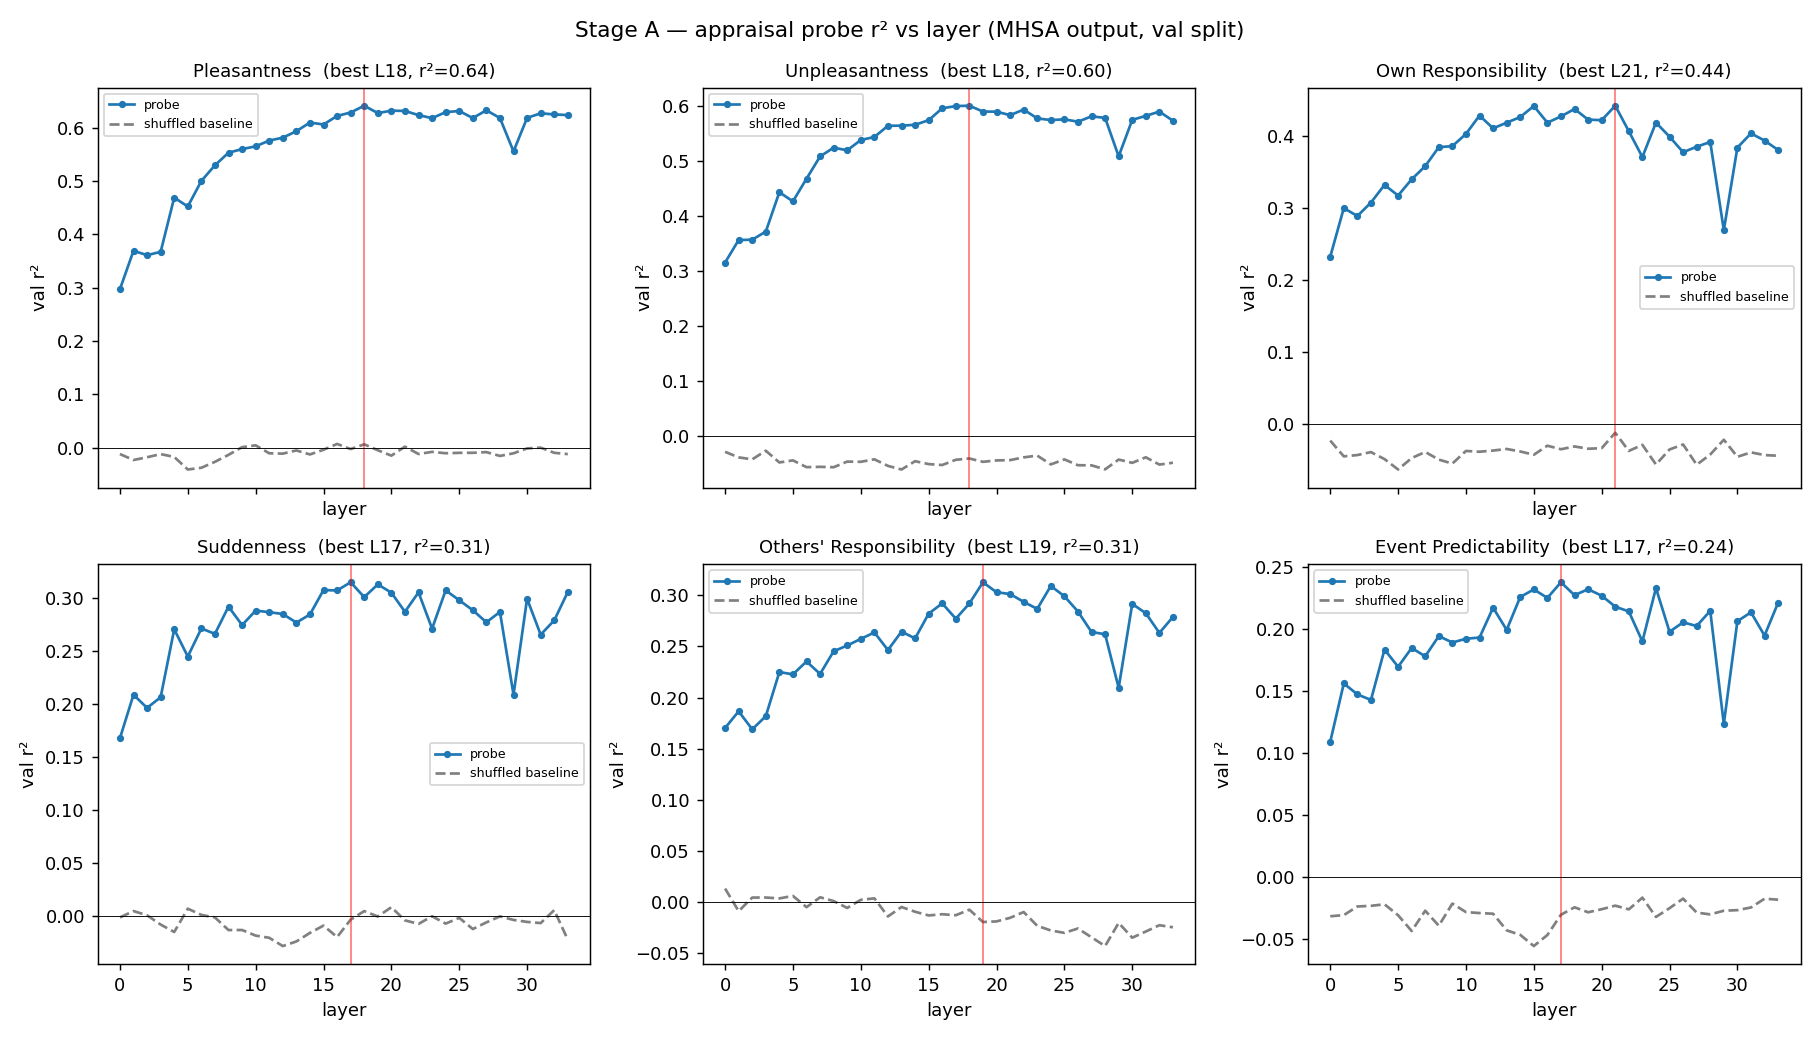
\includegraphics[width=\linewidth]{figures/stage_a_localization.png}
  \end{minipage}\hfill
  \begin{minipage}[t]{0.43\linewidth}
    \centering
    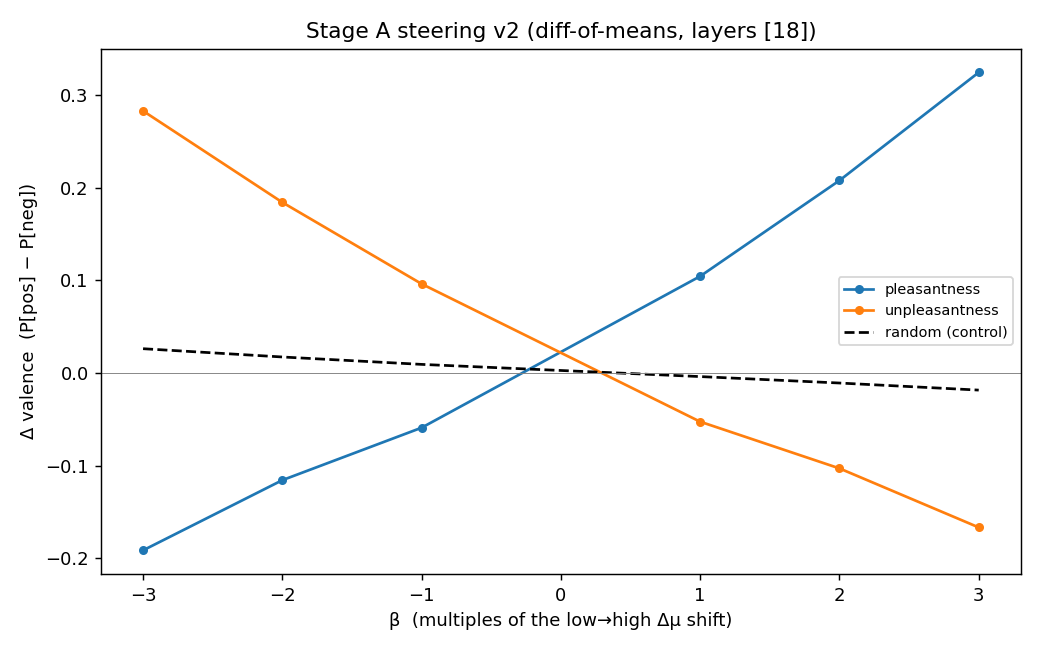
\includegraphics[width=\linewidth]{figures/stage_a_steering_v2.png}
  \end{minipage}
  \caption{Stage A. \emph{Left:} layerwise probe validation $r^2$ per appraisal vs.\ shuffled baselines. \emph{Right:} difference-of-means text steering vs.\ the flat random control.}
  \label{fig:stagea}
\end{figure}

\subsection{Cross-modal readout transfer and caption controls}
Full EMOTIC test split ($n = 7{,}280$): frozen pleasantness probe $\rho = +0.507$ (Pearson $+0.524$), polarity AUC $0.898$ on the 440 single-label images; unpleasantness mirrors ($\rho = -0.448$). The norm-matched random-direction null is nontrivial under anisotropy (100 draws: mean $|\rho| = 0.128$, p95 $= 0.300$, max $= 0.362$); the probe clears all draws (empirical $p = 0.010$). Caption controls (mechanism subset $n = 1{,}000$): unique image contribution $+0.310$ controlling a neutral caption, $+0.256$ a rich perceptual caption, $+0.201$ both jointly (all $p < 0.001$; unpleasantness mirrors at $-0.279 / -0.198 / -0.153$).

\begin{figure}[h]
  \centering
  \begin{minipage}[t]{0.49\linewidth}
    \centering
    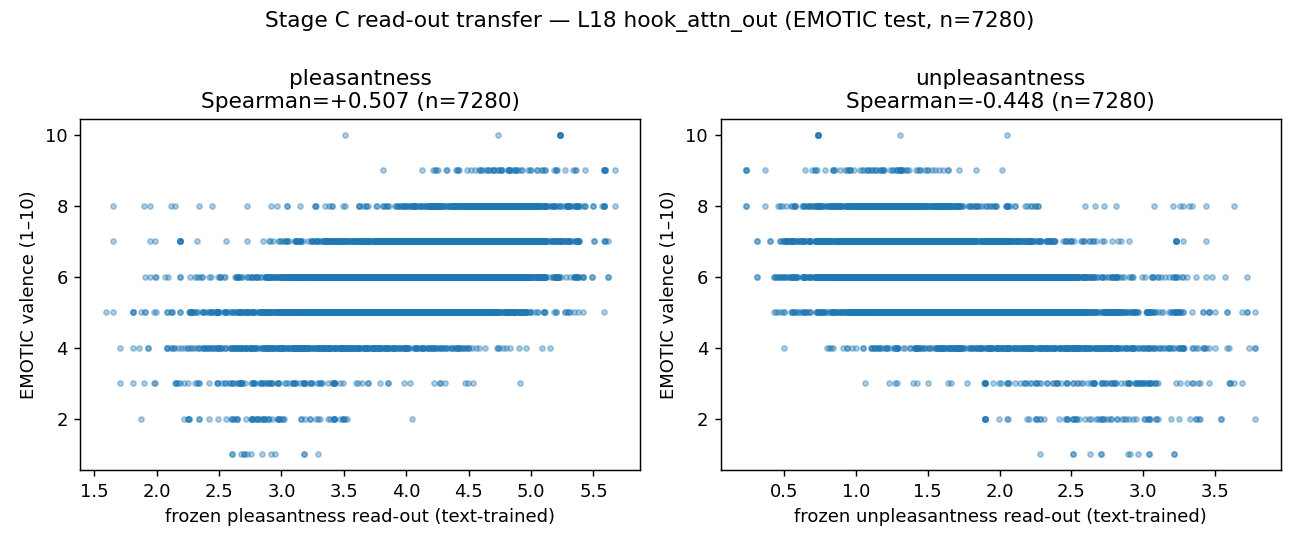
\includegraphics[width=\linewidth]{figures/stage_c_readout.png}
  \end{minipage}\hfill
  \begin{minipage}[t]{0.49\linewidth}
    \centering
    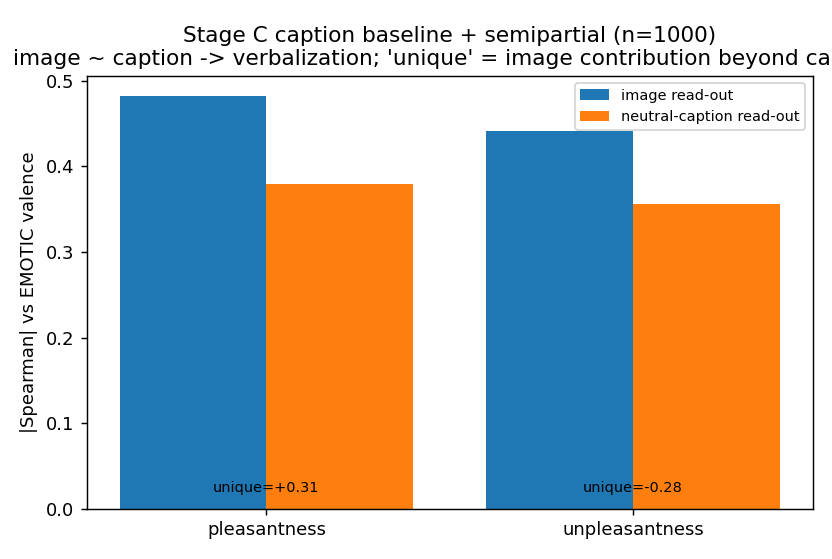
\includegraphics[width=\linewidth]{figures/stage_c_caption_baseline.png}
  \end{minipage}
  \caption{Stage C. \emph{Left:} frozen text-trained probe vs.\ EMOTIC valence under image conditioning. \emph{Right:} caption-control analysis.}
  \label{fig:stagec}
\end{figure}

\subsection{Cross-modal causal steering}
150 EMOTIC test images, steering at resid\_post layer 18 under image conditioning, directions estimated from 1,200 crowd-enVENT train examples (Table~\ref{tab:staged}).

\begin{table}[h]
  \caption{Stage D cross-modal steering: mean $\Delta$ valence vs.\ $\beta$ ($n = 150$ images).}
  \label{tab:staged}
  \centering
  \small
  \begin{tabular}{lrrrrrrr}
    \toprule
    Direction & $\beta{=}{-}3$ & $-2$ & $-1$ & $+1$ & $+2$ & $+3$ & Slope \\
    \midrule
    Pleasantness   & $-1.049$ & $-0.854$ & $-0.466$ & $+0.366$ & $+0.622$ & $+0.762$ & $+0.329$ \\
    Unpleasantness & $+0.716$ & $+0.566$ & $+0.323$ & $-0.412$ & $-0.793$ & $-1.014$ & $-0.309$ \\
    Suddenness (specificity) & $+0.202$ & $+0.138$ & $+0.075$ & $-0.076$ & $-0.156$ & $-0.230$ & $-0.073$ \\
    Random (null)  & $+0.019$ & $+0.037$ & $+0.029$ & $-0.039$ & $-0.088$ & $-0.127$ & $-0.027$ \\
    \bottomrule
  \end{tabular}
\end{table}

\begin{figure}[h]
  \centering
  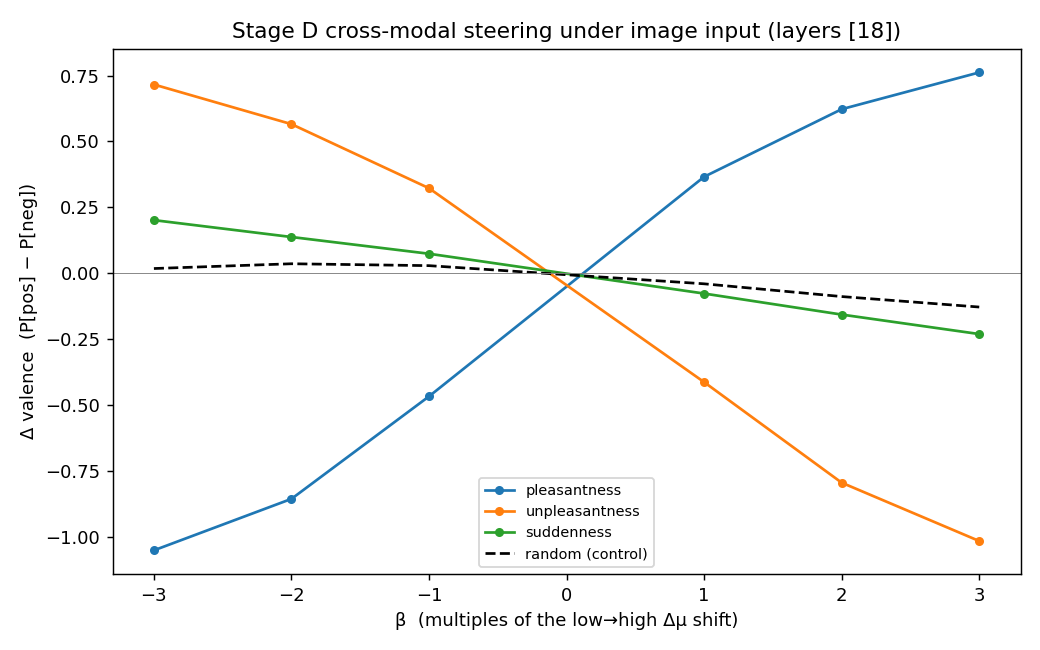
\includegraphics[width=0.65\linewidth]{figures/stage_d_steering.png}
  \caption{Stage D: text-derived appraisal directions steer image-conditioned behavior; controls stay comparatively flat.}
  \label{fig:staged}
\end{figure}

\subsection{Compositional emotion steering (supporting)}
On a 30-image pilot, combinations of text-derived appraisal directions elicit theory-predicted specific emotions. Neither component alone produces anger (unpleasantness alone $\to$ fear; other-responsibility, decorrelated from valence, alone $\to$ joy), but their matched-norm combination makes anger the winning emotion on $97\%$ of images --- the textbook appraisal prediction \emph{anger = negative + other-caused}, realized causally and cross-modally. This result is not load-bearing for the conflict claims; we include it as evidence that the appraisal directions are semantically structured.

\section{Context banks, prompt, and label set}
\label{app:contexts}

\paragraph{Label set.}
The 13 closed-vocabulary emotion labels are anger, boredom, disgust, fear, guilt, joy, pride, relief, sadness, shame, surprise, trust, and neutral; behavioral valence sums P over \{joy, pride, relief, trust\} minus P over \{anger, boredom, disgust, fear, guilt, sadness, shame\}, with surprise and neutral excluded. This partition matches the released code.

\paragraph{Full bank.}
Table~\ref{tab:contextbank} lists the full bank verbatim with each sentence's text-only effect (vs.\ neutral, no image) and mean behavioral valence on the positive-image group. Two negative sentences are weak or mildly positive in isolation (n1 $+0.12$, n4 $-0.42$), consistent with the banks being matched in strength rather than negatives being uniformly extreme.

\begin{table}[h]
  \caption{Full context bank (6 positive, 6 negative, 2 neutral).}
  \label{tab:contextbank}
  \centering
  \small
  \begin{tabular}{llrr}
    \toprule
    ID & ``This photo was taken \ldots'' & Text-only effect & Pos.-img.\ valence \\
    \midrule
    p0 & moments after they won the championship.      & $+0.80$ & $+0.40$ \\
    p1 & at their surprise birthday party.             & $+0.39$ & $+0.15$ \\
    p2 & just after they got the job they wanted.      & $+0.85$ & $-0.18$ \\
    p3 & on the best day of their life.                & $+0.55$ & $-0.13$ \\
    p4 & moments after hearing wonderful news.         & $+0.93$ & $+0.24$ \\
    p5 & at a celebration held in their honor.         & $+0.72$ & $+0.17$ \\
    \midrule
    n0 & moments after they received devastating news. & $-1.07$ & $-0.84$ \\
    n1 & moments before the accident.                  & $+0.12$ & $-0.33$ \\
    n2 & at the funeral of a close friend.             & $-1.02$ & $-0.93$ \\
    n3 & just after they lost their job.               & $-1.06$ & $-0.63$ \\
    n4 & during the worst week of their life.          & $-0.42$ & $-0.57$ \\
    n5 & right after a painful goodbye.                & $-1.06$ & $-0.64$ \\
    \midrule
    z0 & on a weekday.                                 & --- & $+0.05$ \\
    z1 & indoors.                                      & --- & $-0.16$ \\
    \bottomrule
  \end{tabular}
\end{table}

\paragraph{Minimal-pair bank.}
Six pairs, each holding sentence structure and wording constant and flipping only the valence-bearing token; token counts verified equal within each pair on the Gemma tokenizer (per-pair token delta $= 0$, so the readout position is identical within each pair). The exact sentences, with the positive member first (each begins ``This photo was taken \ldots''):
\begin{itemize}\setlength\itemsep{0pt}
  \item[mp0] \ldots moments after they \{won $\mid$ lost\} the championship game.
  \item[mp1] \ldots on the \{best $\mid$ worst\} day of their life.
  \item[mp2] \ldots moments after they \{got $\mid$ lost\} the job they wanted.
  \item[mp3] \ldots moments after they heard \{wonderful $\mid$ devastating\} news.
  \item[mp4] \ldots at a \{celebration $\mid$ memorial\} for a close friend.
  \item[mp5] \ldots during a \{joyful $\mid$ heartbreaking\} moment.
\end{itemize}
Text-only, the minimal banks average $+0.666$ vs.\ $-0.832$ (ratio $1.25$); a couple of positive members read weak in isolation and are flagged for revision.

\paragraph{Prompt.}
The exact template (Gemma chat scaffold; the context part is omitted in the no-context condition):
\begin{quote}\small\ttfamily
<start\_of\_turn>user\textbackslash n<start\_of\_image>Context: \{ctx\} What single emotion is this person feeling?<end\_of\_turn>\textbackslash n<start\_of\_turn>model\textbackslash n
\end{quote}
The readout position is the final prompt token, computed as \texttt{input\_ids.shape[-1] - 1}, never a hardcoded index.

\section{Prompt-variant details}
\label{app:prompts}

\begin{table}[h]
  \caption{Prompt robustness (\gemma{}, full bank, 150 images). The gap is positive with CIs excluding zero under all six phrasings; the base prompt (v0) is mid-pack. v0 reproduces the base run (84/19 vs.\ published 84/21), anchoring the sweep to the original pipeline.}
  \label{tab:prompts}
  \centering
  \scriptsize
  \setlength{\tabcolsep}{3.5pt}
  \begin{tabular}{llrrrr}
    \toprule
    Variant & Phrasing & Neg$>$pos & Pos$>$neg & Gap & 95\% CI \\
    \midrule
    v0 & \emph{What single emotion is this person feeling?} & $84\%$ & $19\%$ & $+65\%$ & $[+0.57, +0.73]$ \\
    v1 & \emph{How is this person feeling?} & $82\%$ & $26\%$ & $+57\%$ & $[+0.47, +0.66]$ \\
    v2 & \emph{In one word, what emotion is this person experiencing?} & $76\%$ & $29\%$ & $+46\%$ & $[+0.37, +0.56]$ \\
    v3 & \emph{What is the most likely emotion of the person in this photo?} & $76\%$ & $27\%$ & $+49\%$ & $[+0.38, +0.60]$ \\
    v4 & context placed after the question & $84\%$ & $29\%$ & $+54\%$ & $[+0.45, +0.63]$ \\
    v5 & bare context sentence, no \texttt{Context:} label & $89\%$ & $16\%$ & $+74\%$ & $[+0.65, +0.81]$ \\
    \bottomrule
  \end{tabular}
\end{table}

\section{The no-context baseline confound}
\label{app:nocontext}

Adding any framing sentence, even a neutral one, raises both readouts relative to the bare no-context prompt (Table~\ref{tab:nocontext}); the shift appears in the frozen probe readout, so it is representational, and it is uniform across the bank. All analyses therefore exclude no-context and baseline against neutral.

\begin{table}[h]
  \caption{Positive-image group, raw means per condition.}
  \label{tab:nocontext}
  \centering
  \begin{tabular}{lrr}
    \toprule
    Condition (positive images) & Behavioral valence & Probe readout \\
    \midrule
    no context           & $-0.469$ & $+4.544$ \\
    $+$ neutral context  & $-0.058$ & $+4.868$ \\
    $+$ positive context & $+0.109$ & $+5.145$ \\
    $+$ negative context & $-0.656$ & $+4.381$ \\
    \bottomrule
  \end{tabular}
\end{table}

\section{Pilot vs.\ full bank}
\label{app:pilot}

A 40-image, one-context-per-polarity pilot reported image dominance (ratio $0.15$--$0.22$) and a large asymmetry that turned out to be artifacts of a single weak positive sentence; the full bank reverses the dominance reading to balanced ($0.86$--$1.19$) and the arbitration slope moves $+0.350 \to +0.215$. We report this as a cautionary result on single-context conflict designs.

\section{Patching methodology}
\label{app:patching}

\paragraph{Same-image design (\S\ref{sec:patching}).}
Donor $=$ positive-context run, recipient $=$ negative-context run, same image; \texttt{resid\_post} overwritten over layers 13--17 for one position-aligned group at a time; recovery $= (\text{patched} - \text{neg})/(\text{pos} - \text{neg})$ at the L18 probe readout. Groups: image (256 tokens), question, BOS, user-turn prefix delimiters, assistant-turn suffix (\texttt{<end\_of\_turn>\textbackslash n<start\_of\_turn>model}); the scoring token itself is excluded from all groups. 60 images per pair; pairs: championship/funeral and wonderful/devastating. Behavioral-valence recovery follows the same ordering but noisier (all-text $73$--$78\%$). Full-bank sentences differ in token length across donor/recipient, so aligned groups sit at different absolute positions; this positional confound is removed by the token-identical minimal pairs, on which the patching rerun is planned.

\paragraph{Cross-image design (\S\ref{sec:crosspatch}).}
Donor $=$ positive image, recipient $=$ negative image, context fixed, so \texttt{input\_ids} are byte-identical and every position is patchable; 60 pairs; bands 0--12, 13--17, 18--28; recovery on behavioral valence, with the L18 probe corroborating where valid (the probe taps \texttt{attn\_out} L18 computed from L17, so probe recovery is invariant-by-construction for the 18--28 band and is gated out there). Sanity: patching all positions except the scoring token recovers $100\%$ / $91\%$ / $79\%$ by band. The negative-context confirmatory run collapses the image-driven gap to $0.08$, making late-band recovery denominators near-zero; its CIs are reported but not interpreted.

\paragraph{Qwen port.}
Raw HuggingFace hooks, behavioral-valence recovery, 60 positive images, broad mid+late band; Qwen distributes the carrier (question $12\%$, turn scaffold $6\%$, all aligned text $65\%$, super-additive), consistent with redundant copies across text positions.

\section{Scale details}
\label{app:scale}

\begin{table}[h]
  \caption{Model-scale comparison (override rates, 121 distinct images, CIs clustered over images). Caveats: the two gap CIs overlap, and at $93\%$ negative override the gap is ceiling-compressed, so no claim is made that the asymmetry changes with scale; the clearly significant change is positive override doubling.}
  \label{tab:scale}
  \centering
  \small
  \begin{tabular}{lrrrrr}
    \toprule
    Model & Params & Neg$>$pos img & Pos$>$neg img & Gap & 95\% CI \\
    \midrule
    \gemma{}    & 4.3B  & $84\%$ & $19\%$ & $+65\%$ & $[+0.57, +0.73]$ \\
    \gemmabig{} & 12.2B & $93\%$ & $42\%$ & $+51\%$ & $[+0.42, +0.59]$ \\
    \bottomrule
  \end{tabular}
\end{table}

\begin{figure}[h]
  \centering
  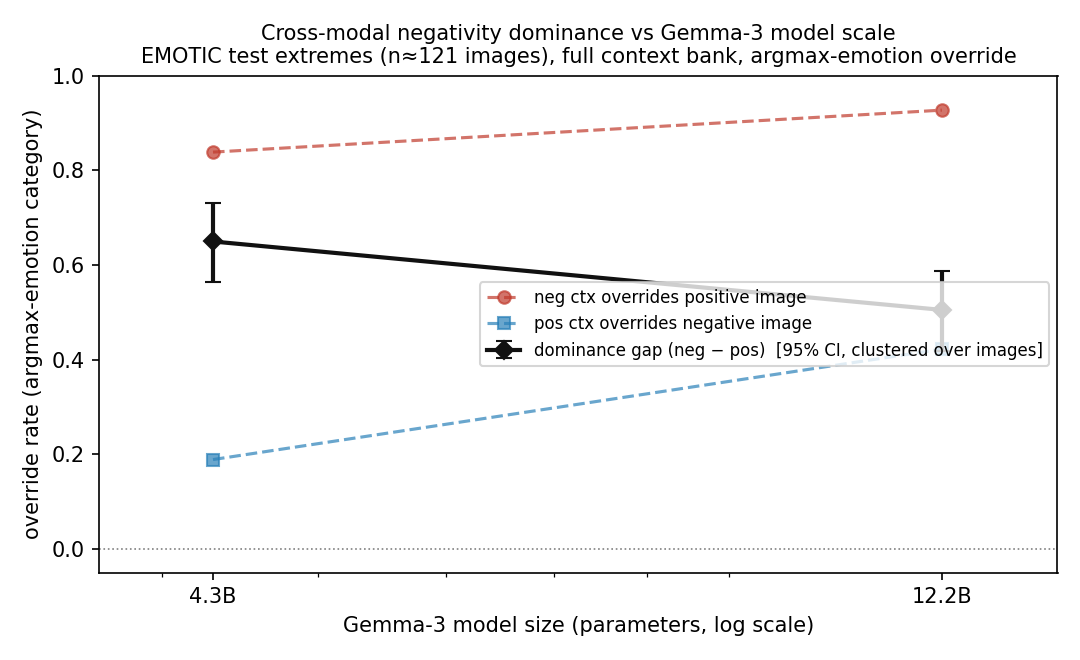
\includegraphics[width=0.7\linewidth]{figures/stage_f_scaling.png}
  \caption{Override rates and dominance gap across Gemma-3 scale.}
  \label{fig:scaling}
\end{figure}

\section{Compute}
\label{app:compute}

All experiments are inference-only single forward passes (no gradients, no generation) on one A100-40GB-class GPU in bf16. Forward-pass counts: full-bank base pass 2{,}250; minimal-pair base pass 2{,}250; text-only controls 15 per bank per model; arbitration sweep 1{,}050; prompt sweep 13{,}500; scaling 2 $\times$ 2{,}250; \qwen{} and \llava{} base passes 2{,}250 each plus text-only; layerwise sweep one cached forward per image per condition pair (51 paired images); same-image patching 60 images $\times$ 2 pairs $\times$ 7 groups; cross-image patching 60 pairs $\times$ 3 bands $\times$ 6 groups plus the negative-context confirmatory run. \todo{Add wall-clock totals per run from the session logs for camera-ready; the full project including preliminary and failed runs used more compute than the reported experiments.}

% ============================================================
\newpage
\input{checklist}

\end{document}
